\documentclass[a4paper]{article}
\usepackage[spanish]{babel}
\title{Taller 1}

\usepackage[utf8]{inputenc}
\usepackage{caratula}
\usepackage{graphicx}
\usepackage{color}
\usepackage{listings}
\usepackage{float}

\setlength{\leftmargin}{2cm}
\setlength{\rightmargin}{2cm}
\setlength{\oddsidemargin}{-1cm}
\setlength{\evensidemargin}{-1cm}
\setlength{\topmargin}{-1cm}
\setlength{\textwidth}{18cm}
\setlength{\textheight}{25cm}

\usepackage{fancyhdr}
\pagestyle{fancy}
\fancyhf{}
\fancyhead[LO,LE]{\scriptsize Trabajo Práctico N$^{\circ}$1}
\fancyhead[RO,RE]{\scriptsize Mancuso, Mataloni, Gonzalez}
\fancyfoot[CE,CO]{\thepage}
\renewcommand{\footrulewidth}{0.4pt}

\usepackage[pdftex, bookmarks=true, colorlinks, citecolor=black, linkcolor=black]{hyperref}
\usepackage{multirow}

\begin{document}

\materia{Teoría de las Comunicaciones}
\submateria{Segundo Cuatrimestre de 2012}
\titulo{Taller de Capa de Enlace}
\grupo{Taller N$^{\circ}$1}

\integrante{Mancuso, Emiliano}{597/07}{emiliano.mancuso@gmail.com}
\integrante{Mataloni, Alejandro}{706/07}{amataloni@gmail.com}
\integrante{Gonzalez, Matias}{453/07}{curtu\_infinito73@hotmail.com}

\maketitle

\newpage

\addcontentsline{toc}{section}{Índice}
\tableofcontents

% Main project

\beg

\newpage

\section{Primera consigna}

Utilizamos \textit{Scapy} para implementar un pequeño script que, dada una dirección IP, realiza un pedido por la MAC Address y muestra en pantalla la respuesta en caso de recibir alguna.\\

El script es el siguiente:

\begin{verbatim}
	pkt = ARP(pdst=sys.argv[1], op="who-has");
	response = sr1(pkt)
	response.show()
\end{verbatim}

Lo interesante es ver que ocurre en algunos casos:

\begin{itemize}
\item dirección inexistente = el script se cuelga esperando la respuesta que nunca llega. 
\item dirección de la maquina de origen = el paquete ARP no se envía.
\item dirección Broadcast = pregunta por la dirección por lo que pasa lo mismo que si fuera una dirección inexistente 
\item dirección de red = pregunta por la dirección por lo que pasa lo mismo que si fuera una dirección inexistente 
\end{itemize}


\section{Segunda consigna}

Implementamos un script en \textit{Scapy} para escuchar pasivamente en la red y capturar cada mensaje ARP enviado. En el mismo script cuando capturamos el mensaje, traducimos los datos del \textit{vendors} y los imprimimos por pantalla.\\

El script es el siguiente:

\begin{verbatim}
  # Print pretty vendor
  def arp_monitor_callback(pkt):
    vendor_prefix = pkt[ARP].hwsrc[0:8].upper()
    strr =  pkt[ARP].psrc + ": \t" + vendors_dict[vendor_prefix]
    print strr


  # Build the vendor dictionary
  ins = open("vendorsUtil.txt", "r")
  vendors_dict = {}
  for line in ins:
    vendors_dict[line[0:8]] = line[9:-1] 
   
  ins.close()
	
  if len(sys.argv) == 1:
    print "Listening for 5 seconds.."
    to = 5  # Default value
  else:
    to = int(sys.argv[1]) 

  sniff(prn=arp_monitor_callback, filter="arp", store=0, timeout=to)	
\end{verbatim}

\newpage

\section{Tercera consigna}

Para esta parte lo que hicimos fue capturar los paquetes \textit{ARP}, y crear un grafo dirigido de IPs. Cada nodo representa una dirección IP y existe un eje entre dos nodos \textit{x} e \textit{y} si y solo si, se observo un request ARP con \textbf{source} \= IP de \textit{x} y \textbf{target} \= IP de \textit{y}. 
 Consideramos que esta es la mejor forma para extraer información en cuanto a la topología de la red en cuestión, así como también sacar datos interesantes de la misma. \\
 

\begin{figure}[H]
  \centering
  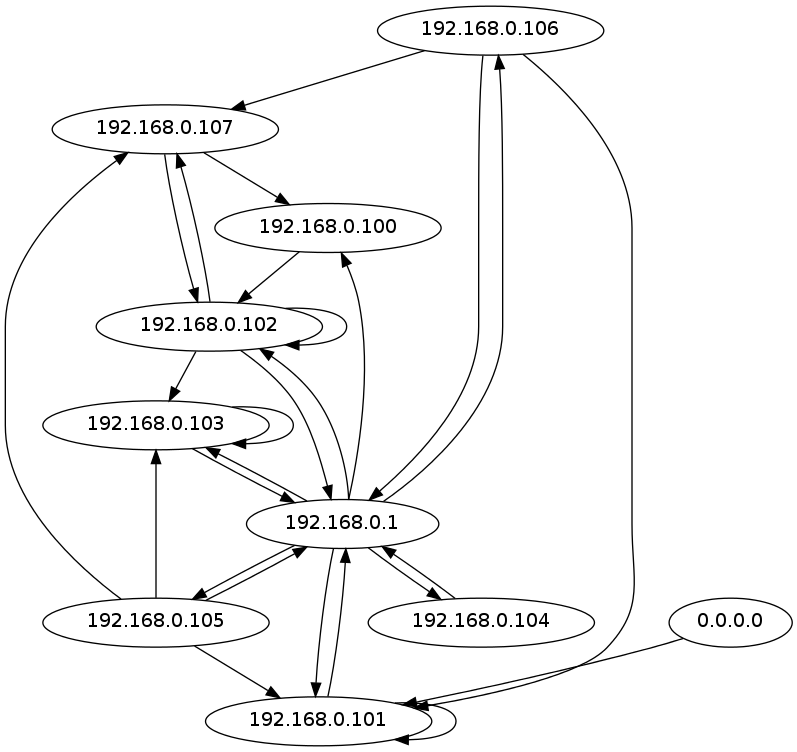
\includegraphics[scale=0.30]{graficos/arpGraph.png}
  \caption{Gráfico dirigido de los distintos request ARP observados.}
\end{figure}

 
La muestra fue obtenida de la casa de uno de los integrantes del grupo y la finalizamos al alcanzar los 300 paquetes ARP.  
Si bien es una red pequeña pensamos que para este taller en particular al trabajar con paquetes ARP no influía tanto la cantidad de dispositivos.

Inmediatamente nos damos cuenta que la IP 192.168.0.1 es la asignada al router, ya que ésta es la que más se comunica con el resto de los dispositivos. 
Otro caso interesante a estudiar es el de los nodos que tienen ejes dirigidos a si mismos. Esto sucede en los paquetes ARP que son del tipo \textit{gratuitous}. Este tipo de paquetes se mandan generalmente cuando un dispositivo se conecta a la red, avisando al resto de su ubicación. Son útiles también para: detectar IPs repetidas.

Otro caso significativo el el nodo con IP 0.0.0.0, la cual no es una dirección válida. No pudimos saber con exactitud por que sucedió pero por lo que investigamos se pude deber a que el dispositivo envió el request antes de que se le haya asignado una IP válida. 


 



\end{document}
